\section{Shellcode}
\subsection{Definition}
Um den nächsten Teil besser zu verstehen, sollte vorher erklärt werden, was genau Shellcode ist, wofür er 
benutzt wird und was der Zusammenhang zur Assembler Programmiersprache ist. Shellcode ist definiert als eine 
Reihe von Anweisungen, die über einen Exploit injiziert und dann durch den Prozess ausgeführt werden.
Shellcode wird verwendet, um Register direkt zu manipulieren und die Funktionalität eines Programms auszunutzen. 
Es ist natürlich möglich, Shellcode in höheren Programmiersprachen zu schreiben, aber die effizienteste und fast 
ausschließlich benutzte Variante ist in der Sprache Assembly, die so maschinennah wie möglich ist, um genau steuern 
zu können was passiert und Speichergröße zu sparen. Meistens arbeitet man nämlich mit einer limitierten Speichergröße.
In der Computersicherheit bedeutet Shellcoding im wahrsten Sinne des Wortes das Schreiben von Code, der bei der
Ausführung eine Remote-Shell zurückgibt. Die Bedeutung von Shellcode hat sich weiterentwickelt und stellt nun jeden
Byte-Code dar, der in einen Exploit eingefügt wird, um eine gewünschte Aufgabe zu erfüllen. Da Shellcode in Assembly
geschrieben wird und die Sprache so maschinennah wie nur möglich ist, ist es außerdem noch wichtig mit welcher
Hardware und mit welchem Betriebssystem man diese schreibt. Es bestehen nämlich Unterschiede zwischen Linux
Shellcode und Windows Shellcode:  Bei Linux hat man direkten Zugriff auf das Interface und das Kernel, was bei
Windows leider nicht möglich ist. Im folgenden Beispiel wird ein Shellcode-Beispiel in der Sprache Assembly erläutert.
Die Idee hinter dem Beispiel ist es, zu zeigen, wie man mit einem Buffer Overflow Zugriff bekommen kann und dann den
vorbereiteten Shellcode injizieren kann, damit dieser privilegiert ausgeführt wird und somit Schaden am Ziel verursacht.

\subsection{Beispiel}
\begin{figure}[h]
    \centering
    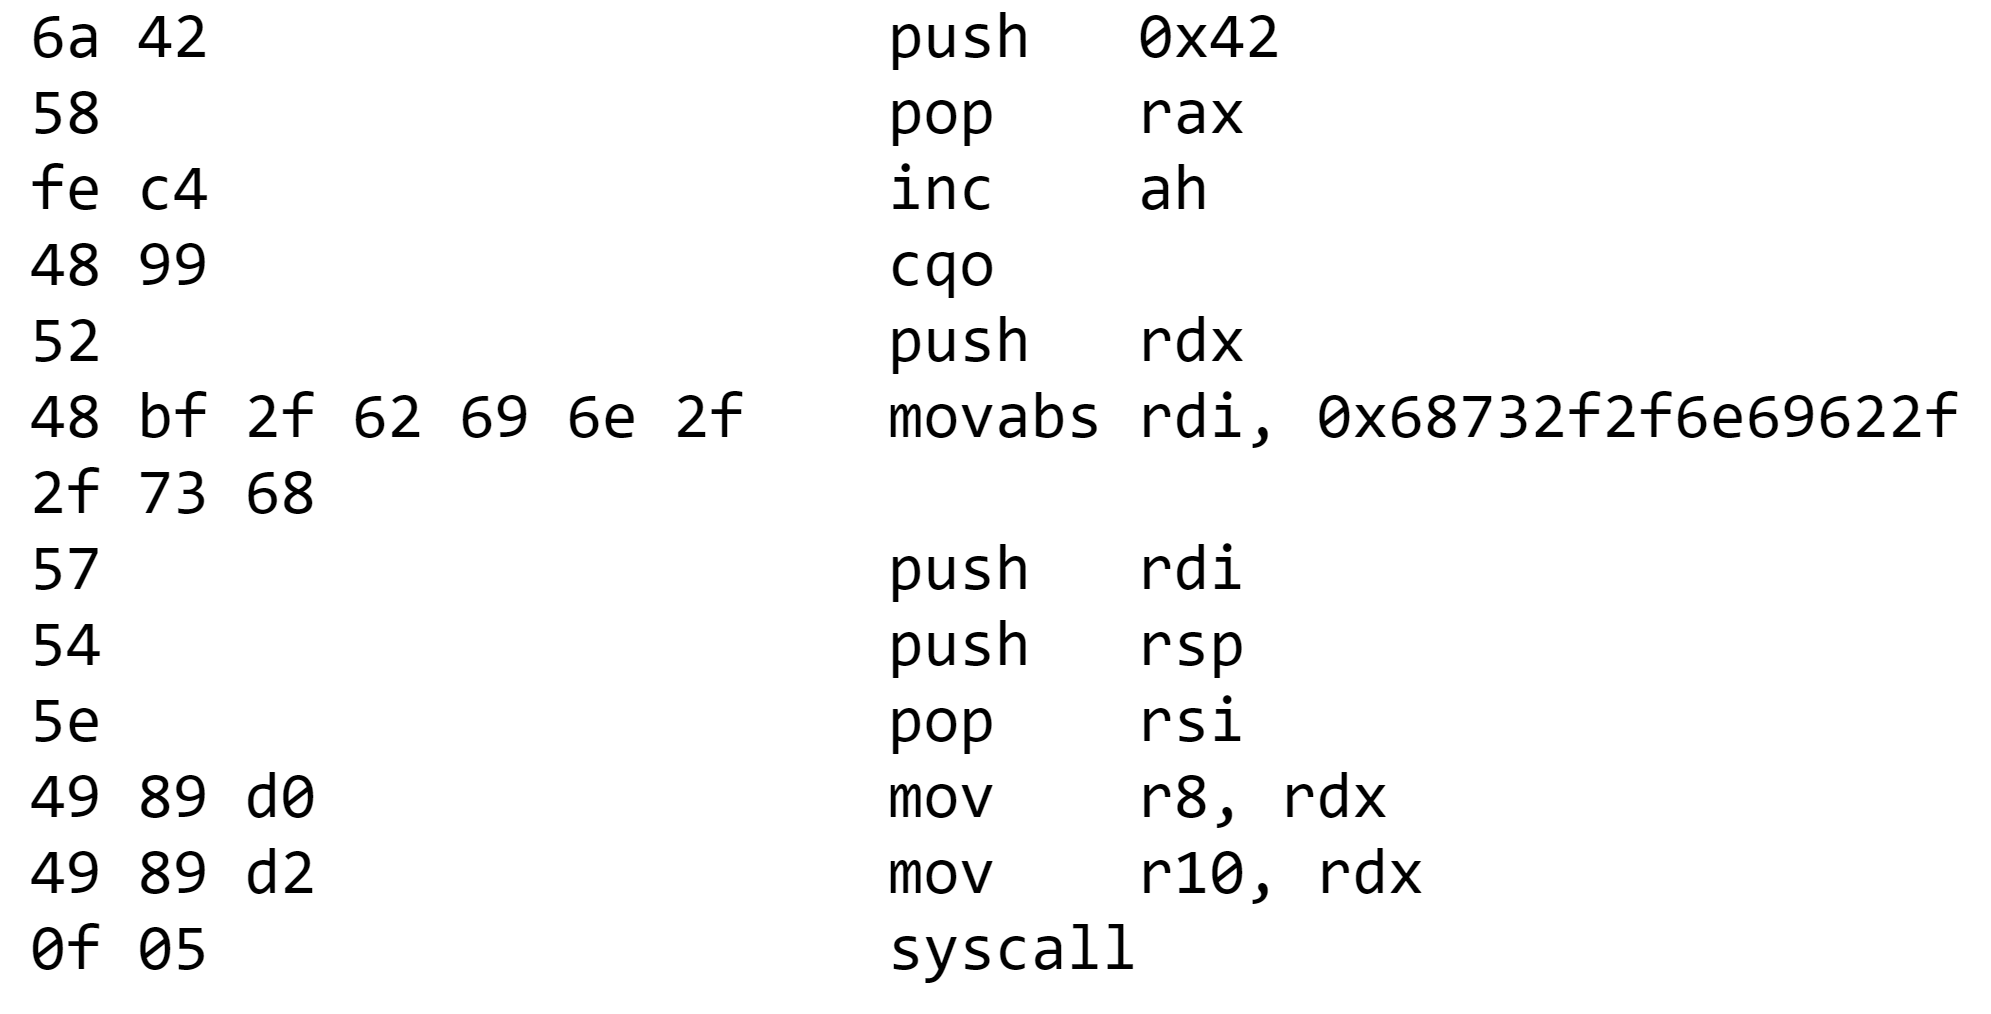
\includegraphics[width=0.9\textwidth,height=0.75\textheight,keepaspectratio]{images/shellstorm.png}
    \caption{Shellcode}
\end{figure}

%TODO: Einfügen aus DC
%Struktur:
%Der syscall wird abgeschickt, vorher müssen einige Werte gesetzt werden um execveat aufzurufen



RAX -> system call number (322) 
RDI -> first argument (path)
RSI -> second argument (pointer to path)
RDX -> third argument (0)
R10 -> fourth argument(0)
R8 -> fifth argument(0)
R9 -> sixth argument (not used) (Bearbeitet)


Bei dem folgenden Bild sieht man ein Beispiel zu einem Shellcode der dann wenn man
%!!!
vorhat ausgeführt werden kann um ein System zu manipulieren.Dieses ist aber einfach
gehalten um einen übersichtlicheren Blick zu bekommen. Daher sollte man hier von unten
beginnen. Der System Call wird aufgerufen und geht an die Adresse im Register RAX.
Dieser wurde mit der Hexadezimalzahl 0x42 belegt die auf den Stack gepusht
war und durch das pop da eingespeichert wurde, wichtig hierbei ist dass,
danach das Register ah was ein 8 Bit Teil vom 64 Bit Register RAX ist inkrementiert wird.
Mit anderen Worten wird der Wert 0x42 zum Wert 0x142 dieser ist in
Dezimalzahlen 322.Also geht der  System Call an die Nummer 322.
Der nächste Schritt des Aufrufs ist es ans Register RDI zu gehen was das first
argument enthält und den path darstellt. Im Code sehen wir das durch den
Befehl movabs der String ("/bin//sh") als Hexadezimalzahl ins Register
verschoben wird und danach durch den push Befehl auf dem Stack ist.
Der dritte Schritt ist dass, der Aufruf sich das second argument anguckt
was den Weg zum path hat und im Register RSI enthalten ist. Das besondere
Register RSP oder auch stack pointer zeigt auf den Pfad der letzten Adresse
in dem falle den von RDI und dieser Pfad wird in RSI gespeichert, daher die
Befehle push RSP und pop RSI. Der Rest vom Code ist in diesem falle nicht so
wichtig aber durch den Befehl cqo(convert word to Quadword) am Anfang wird das
Register RDX auf null gesetzt und diesen Wert übernehmen dann auch die zwischen
Register R8 und R10 durch den mov Befehl. Einen wirklichen nutzen hat dieser
kleine 29 Byte große
Shellcode nicht, aber er zeigt hervorragend wie man die Register mit dem der
Kernel durch den System Call arbeitet man manipulieren kann.
